\documentclass[11pt]{article}
\usepackage[margin=1in]{geometry}
\usepackage{amsmath,amssymb,amsthm}
\usepackage{booktabs}
\usepackage{graphicx}
\usepackage[numbers,sort]{natbib}
\usepackage{xurl}
\usepackage[hidelinks]{hyperref}
\usepackage[T1]{fontenc}
\usepackage{lmodern}
\usepackage{microtype}

\newtheorem{proposition}{Proposition}
\newtheorem{corollary}{Corollary}
\theoremstyle{remark}
\newtheorem{remark}{Remark}
\DeclareMathOperator{\E}{E}
\newcommand{\ceil}[1]{\lceil #1 \rceil}
\newcommand{\floor}[1]{\lfloor #1 \rfloor}

\title{The Ninetieth Percentile Is the Maximum:\\ Order-Statistic Bias in the 2026 CMS Hospital Allowed-Amount Rule}
\author{Tristan Kennedy\\ Department of Mathematics and Statistics\\ Virginia Commonwealth University\\ \texttt{tristan@tristkenn.com}}
\date{Preprint, October 2026. Not peer reviewed.}

\begin{document}
\maketitle

\begin{abstract}
Since 2026, US hospitals must publish the median, 10th and 90th percentile of the amounts insurers actually paid them. When a percentile falls between two observed payments, the regulation says to report the next highest one.

We find that the rule is under-specified. Readings consistent with CMS's own gloss pick different order statistics at the 10th percentile for 80\% of sample sizes, and one common reading also differs at the 90th for 79\%. Under every such reading, for counts of 10 or fewer, the published 90th percentile is the sample maximum. Those counts are published only as ``1 through 10''.

We measure this in 1.16 million populated cells from the price files of a stratified random sample of 300 US hospitals. In the average file, 75.5\% of cells (95\% CI 72.6--78.4) have masked counts. In 39.2\% (35.9--42.7), the published 90th percentile is either a maximum over distinct values or carries an estimated upward bias from the rule above 1\%. In 8 of 91 files, some published per-case percentiles fall between cents, so they cannot be observed payments, which suggests interpolation.

Using classical spacing results, we show that under the default type-7 reading the rule never lowers an estimate. Its expected excess over the type-7 quantile is $\delta_n/\{(n+1)f(Q(p))\}+O(n^{-2})$, where $\delta_n$ is a rounding gap that depends only on $n$. We also give a correction that uses only the published summary, state what that summary cannot recover, and recommend specifying the estimator by rank.
\end{abstract}

\section{Introduction}

The calendar-year 2026 Outpatient Prospective Payment System final rule changed what US hospitals must publish about their prices \citep{fr2025}. For each payer and service whose negotiated rate is set as a percentage of charges or by an algorithm, a hospital's machine-readable file must now report four numbers. Three come from its remittance (EDI 835) data over a 12-to-15-month lookback: the median, 10th percentile and 90th percentile of allowed amounts. The fourth is the count of those amounts. Enforcement began on April 1, 2026. These fields are meant to let patients, employers and researchers see the realized price distribution behind an opaque contract term.

The regulation also says how to compute the percentiles \citep{ecfr180}:
\begin{quote}
``Should the calculated median fall between two observed allowed amounts, the median allowed amount is the next highest observed value.''
\end{quote}
The 10th and 90th percentile definitions use the same wording. Commenters objected that this departs from the standard calculation and would need custom formulas. CMS kept the rule so that every published figure is an amount a hospital actually received \citep[][at 53990]{fr2025,hfma2025}. CMS's FAQ warns that the definitions ``may require that the values be calculated in a fashion that may differ from typical arithmetic convention'' \citep{cmsfaq}. Counts from 1 to 10 are published only as ``1 through 10'', following CMS's cell-suppression policy. The percentiles themselves are still published for those cells \citep{cmsdd}.

That the rule is non-standard is therefore known. This note asks how far it departs from standard, in which direction, and in how much of the published data. Our contributions are:
\begin{enumerate}
\item \emph{The ambiguity, quantified.} The rule's own gloss fixes only the median. Readings consistent with it select different order statistics at the 10th percentile for 80\% of $n$, and one of them also at the 90th for 79\%. Under all of them the published 90th percentile is the maximum whenever the count is masked (Section~\ref{sec:rule}).
\item \emph{Exposure and compliance in real files.} In a probability sample of hospitals, we measure how many published cells are masked, tied or exposed to material bias, and how many publish values that cannot be observed payments (Section~\ref{sec:empirical}).
\item \emph{Bias, from classical results.} Using standard spacing identities \citep{pyke1965,davidnagaraja2003,jonesbalakrishnan2002}, the rule's excess over the type-7 quantile is a fixed fraction of one sample spacing and is never negative. We give its expectation, first-order size, and the exact expected content of the published 10--90 band (Section~\ref{sec:bias}).
\item \emph{A correction and its limits.} Recovering a quantile from a few published order statistics is the same problem meta-analysts face when estimating a mean and SD from reported quantiles \citep{hozo2005,wan2014,luo2018,mcgrath2020}. We adapt a log-linear version and list what cannot be recovered (Section~\ref{sec:recover}).
\end{enumerate}

Peterson-KFF \citep{kff2026} report that the count was zero in 92--95\% of commercial percentage and algorithm rates in schema-compliant files. They do not examine how the percentiles are computed. Their denominator is all such rates. Ours is the much smaller set of populated cells, so the two sets of numbers measure different things.

The question matters beyond consumer comparisons. In a game-theoretic model of disclosure format, Ak\c{c}ura and \"{O}zdemir \citep{akcura2026} treat the published percentile spread as ``a deterministic reflection of the rate's true dispersion'' that a regulator can screen on. Sections~\ref{sec:bias} and~\ref{sec:empirical} show that at the counts most cells actually have, the spread is a biased and reading-dependent statistic.

\section{The rule as an order statistic}\label{sec:rule}

Let $X_{(1)}\le\dots\le X_{(n)}$ be the $n$ allowed amounts for one cell, sorted, and let $0<p<1$. Hyndman and Fan \citep{hyndmanfan1996} write the common sample quantiles as $(1-g)X_{(j)}+gX_{(j+1)}$ with $h$ a position, $j=\floor{h}$ and $g=h-j$. Type~7, the default in R, NumPy and Excel's \texttt{PERCENTILE.INC}, uses $h=(n-1)p+1$. The rule does not name a position. It says only that, when the ``calculated'' percentile falls between two observations, the larger is reported. Its one worked gloss is that this happens for the median exactly when $n$ is even \citep[][at 53993]{fr2025}. Any position with $h(n,\tfrac12)=(n+1)/2$ satisfies that gloss, which includes types 5 to 9. We take type~7 as the primary reading because it is the out-of-the-box computation the commenters referred to:
\begin{equation}\label{eq:cms}
\widehat Q^{\mathrm{CMS}}_p = X_{(k)},\qquad k=k_n(p)=\ceil{(n-1)p}+1 .
\end{equation}
This is NumPy's \texttt{method="higher"}.

\begin{proposition}\label{prop:type1}
Let $\widehat F_n^{-1}(q)=X_{(\ceil{nq})}$ be the inverse empirical CDF (type 1). Then $\widehat Q^{\mathrm{CMS}}_p=\widehat F_n^{-1}\{p+(1-p)/n\}$. For $n\ge 3$, $\widehat Q^{\mathrm{CMS}}_p$, viewed as a function of $p$, is none of the nine Hyndman--Fan types.
\end{proposition}

The first claim is the identity $(n-1)p+1=n\{p+(1-p)/n\}$. For the second, as a function of $p$, \eqref{eq:cms} is a step function that jumps at $p=i/(n-1)$. Types 1 and 2 jump at $i/n$, and type 3 jumps near $(i-\tfrac12)/n$. Types 4 to 9 are continuous in $p$.

The rank in \eqref{eq:cms} is never below the type-1 rank $\ceil{np}$ and exceeds it by at most one. At the median, $k=\floor{n/2}+1$, the upper median. For $2\le n\le 11$ the published 10th percentile is $X_{(2)}$. Software differences of this kind are a known teaching problem \citep{langford2006}.

\paragraph{Under-specification at the tails.} Two other readings satisfy the gloss. One takes the ceiling of the type-6 position, $k=\min\{\max(\ceil{(n+1)p},1),n\}$, as in SPSS and Excel's \texttt{PERCENTILE.EXC}. The other takes the upper inverse ECDF, $k=\floor{np}+1$. All three agree at the median for every $n$.

At the tails they diverge, counting over $n\in\{1,\dots,1000\}$. The type-6 reading differs from \eqref{eq:cms} by one rank for 80\% of $n$ at the 10th percentile and 79\% at the 90th. The upper-ECDF reading agrees with \eqref{eq:cms} at the 90th percentile but differs at the 10th for 80\% of $n$. Two hospitals can follow the regulation, start from identical payments and publish different order statistics.

\paragraph{Masked cells.} Under all three readings, $k_n(0.9)=n$ for every $n\le10$. \emph{In every masked cell the published 90th percentile is the largest payment.} Plain type~1, $\ceil{np}$, would give $X_{(9)}$ at $n=10$. But type~1 reports the lower median for even $n$, which the gloss rules out.

\section{Bias}\label{sec:bias}

Write $h=(n-1)p+1$, $j=\floor{h}$, $g=h-j$, and the \emph{rounding gap}
\[
\delta_n(p)=\ceil{h}-h\in[0,1).
\]
For $p=0.9$, $\delta_n=((n-1)\bmod 10)/10$. For the median, $\delta_n=\tfrac12$ for even $n$ and $0$ for odd $n$. Let $S_j=X_{(j+1)}-X_{(j)}$ be the $j$th spacing and $T_7=(1-g)X_{(j)}+gX_{(j+1)}$.

\begin{proposition}[pathwise excess]\label{prop:path}
On every sample, $\widehat Q^{\mathrm{CMS}}_p-T_7=\delta_n(p)\,S_j\ge 0$.
\end{proposition}

If $g=0$, both estimators equal $X_{(j)}$ and $\delta_n=0$. Otherwise $\ceil{h}=j+1$, and $X_{(j+1)}-T_7=(1-g)S_j=\delta_nS_j$. The rule therefore never lowers an estimate, so its error does not average out across cells.

\begin{proposition}[expected excess]\label{prop:spacing}
Let $X$ have an absolutely continuous quantile function $Q$ on $(0,1)$ with $\E X_{(j+1)}<\infty$. Then
\[
\E\big[\widehat Q^{\mathrm{CMS}}_p-T_7\big]=\frac{\delta_n(p)}{n+1}\,\E\,Q'(V),\qquad V\sim\mathrm{Beta}(j+1,\,n-j+1).
\]
If in addition $Q'$ is twice continuously differentiable near $p$ and $\E Q'(V)$ admits the usual delta-method expansion, then
\[
\E\big[\widehat Q^{\mathrm{CMS}}_p-T_7\big]=\frac{\delta_n(p)}{(n+1)\,f\{Q(p)\}}+O(n^{-2}).
\]
\end{proposition}

The proof is in Appendix~\ref{app:proofs}. The identity behind it, $\E S_j=\E Q'(V)/(n+1)$, is a change of variables in the classical expression for expected spacings \citep{pyke1965,jonesbalakrishnan2002}. What is new here is only its application to the rule. For lognormal data with log-scale $\sigma$, $Q(p)f\{Q(p)\}=\phi(z_p)/\sigma$, so the relative excess is approximately
\begin{equation}\label{eq:lognormal}
\frac{\delta_n(p)\,\sigma}{(n+1)\,\phi(z_p)} .
\end{equation}
At $p=0.9$, $\sigma=0.8$ and $n=30$ ($\delta=0.9$), \eqref{eq:lognormal} gives 13.2\%; the exact value is 14.3\%.

Against the true quantile, the standard expansion of $\E X_{(k)}$ \citep[\S4.6]{davidnagaraja2003} gives
\[
\operatorname{Bias}\big(\widehat Q^{\mathrm{CMS}}_p\big)=\frac{(1-2p+\delta_n)\,Q'(p)+\tfrac12p(1-p)\,Q''(p)}{n}+O(n^{-2}),
\]
which is the type-7 bias plus the rule's $\delta_nQ'(p)/n$. At the 90th percentile, type~7's first-order term is negative ($1-2p=-0.8$). The rule's $+\delta_n$, up to $+0.9$, cancels it and then some, and a convex upper tail ($Q''>0$) pushes the total further up.

\begin{proposition}[band content]\label{prop:band}
For continuous $F$, $\E\big[F(\widehat P_{90})-F(\widehat P_{10})\big]=\{k_n(0.9)-k_n(0.1)\}/(n+1)$.
\end{proposition}

This follows from $F(X_{(k)})\sim\mathrm{Beta}(k,n-k+1)$. Under \eqref{eq:cms} the published 10--90 band covers on average 72.7\% of the payment distribution at $n=10$, 77.4\% at $n=30$ and 79.2\% at $n=100$, against a nominal 80\%.

\begin{remark}[ties]
Payment data has many ties. Contracted fee-schedule payments repeat exactly. CMS also tells hospitals to divide time-based payments by the number of units and enter each unit as a repeated observation \citep[p.~13]{cmsfaq}. When a quantile sits inside a run of tied values, $S_j=0$ and the rule changes nothing, so the continuous-$F$ results above apply only to the untied part of the data. Published values give a sandwich test. If $\hat m=\hat P_{90}$, every order statistic between ranks $k_n(0.5)$ and $k_n(0.9)$ is equal, so the rule's 90th-percentile excess is exactly zero. We use this in Section~\ref{sec:empirical}.
\end{remark}

\section{Simulation}\label{sec:sim}

\paragraph{Protocol.} Bias is computed rather than simulated. The expected value of each order statistic is $\E X_{(k)}=\int_0^1 Q\{I^{-1}(t;k,n-k+1)\}\,dt$, evaluated by a 1000-node midpoint rule for every $n=1,\dots,1000$. Root mean squared error and the corrected estimator use Monte Carlo with 10{,}000 replicates per $n$. The Monte Carlo bias matches the exact bias to within about two Monte Carlo standard errors. There are four distributions, all scale-free:
\begin{itemize}
\item lognormal with $\sigma=0.3$ and $\sigma=0.8$;
\item gamma with shape 2;
\item a \emph{contract mixture}. It has atoms at 0.80 (10\%), 1.00 (50\%, the fee-schedule rate) and 1.04 (20\%, a renegotiated rate, since CMS requires pooling across renegotiation \citep{cmswebinar}), plus a 20\% continuous lognormal$(\log1.3,0.5)$ tail.
\end{itemize}
Code and output are in the replication files.

Figure~\ref{fig:bias} shows the excess $\E[\widehat Q^{\mathrm{CMS}}_p-T_7]/Q(p)$. Its sawtooth follows $\delta_n$: at the 90th percentile it peaks at $n\equiv 0\pmod{10}$ and vanishes at $n\equiv1\pmod{10}$. Table~\ref{tab:bias} reports the largest $n$ at which the excess still exceeds 1\% and 5\%.

\begin{figure}[t]
\centering
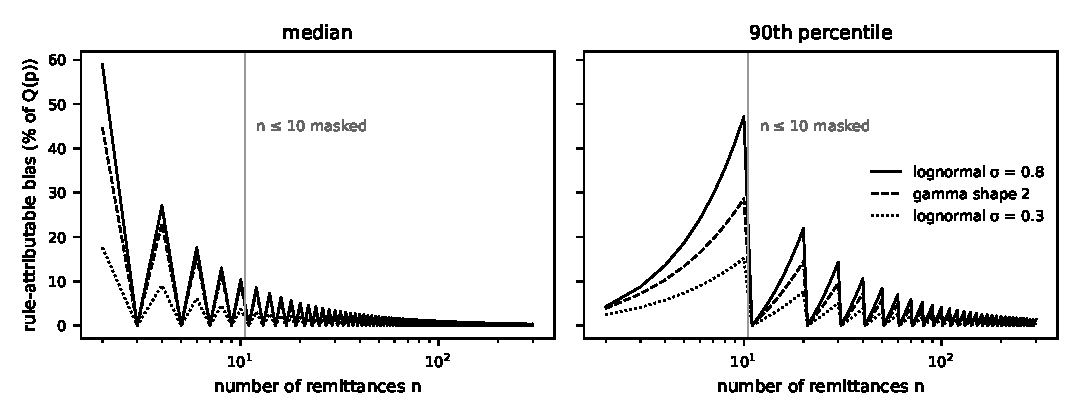
\includegraphics[width=\linewidth]{fig_bias.pdf}
\caption{Rule-attributable relative bias $\E[\widehat Q^{\mathrm{CMS}}_p-T_7]/Q(p)$, exact, $n=2,\dots,300$ (log scale). Counts left of the grey line are published as ``1 through 10''.}
\label{fig:bias}
\end{figure}

\begin{table}[t]
\centering
\caption{Rule-attributable relative bias $\E[\widehat Q^{\mathrm{CMS}}_p-T_7]/Q(p)$ in \%, at $n=10/30/100/500$, and the largest $n\le1000$ at which it exceeds 1\% and 5\%. These four $n$ are the worst rounding phase at the 90th percentile ($\delta=0.9$).}
\label{tab:bias}
\begin{tabular}{llcc}
\toprule
Distribution & Quantile & Bias at $n=10/30/100/500$ & Last $n$ with $>1\%$ / $>5\%$\\
\midrule
Lognormal $\sigma=0.3$ & median & 3.7 / 1.2 / 0.4 / 0.1 & 36 / 6\\
 & 90th & 15.2 / 5.1 / 1.5 / 0.3 & 150 / 30\\
Lognormal $\sigma=0.8$ & median & 10.3 / 3.4 / 1.0 / 0.2 & 100 / 20\\
 & 90th & 47.2 / 14.3 / 4.2 / 0.8 & 410 / 80\\
Gamma, shape 2 & median & 9.4 / 3.2 / 0.9 / 0.2 & 94 / 18\\
 & 90th & 28.7 / 9.6 / 2.9 / 0.6 & 290 / 50\\
Contract mixture & median & 0.4 / 0.1 / 0.0 / 0.0 & 6 / 2\\
 & 90th & 40.1 / 14.1 / 4.9 / 1.1 & 560 / 90\\
\bottomrule
\end{tabular}
\end{table}

Per cell, sampling error is larger than the rule's bias once $n\ge30$. At $\sigma=0.8$, $n=30$, the 90th-percentile RMSE is 31\% under the rule against 23\% for type~7, and the two are within 2 points at $n=100$. The case for caring about the rule therefore rests on aggregation and comparability, not on any single cell. The bias has one sign, so it survives averaging across cells, hospitals and payers. Because of the tail ambiguity above, it also differs between hospitals that read the rule differently.

\section{Exposure in published files}\label{sec:empirical}

\paragraph{Data.} The frame is the 4{,}397 non-federal acute-care and critical-access hospitals in CMS Hospital General Information. We drew 300 at random within strata of Census region by hospital type, with proportional allocation. For each sampled hospital we fetched its \texttt{cms-hpt.txt} index and price file on October 17, 2026, reading up to 300 MB of each file. A \emph{populated cell} is a payer-level row with a nonzero median backed by a nonzero count. That gives 1{,}158{,}679 populated cells in 167 distinct files. Hospitals that populate the fields are a minority \citep{kff2026}, so the results below describe published cells, not hospitals in general. Files are the unit: each file gets equal weight, which stops a few very large files from dominating, and intervals are percentile bootstraps over files ($B=2000$).

\paragraph{Plug-in exposure.} For cells with a known count ($n\ge11$) we estimate the rule-attributable bias at the 90th percentile and the median from \eqref{eq:lognormal}. In it we use $\hat\sigma=\log(\hat P_{90}/\hat P_{10})/2.563$, the lognormal scale implied by the published band. This is a first-order, shape-dependent approximation. It also uses the published, rule-affected band itself, which inflates $\hat\sigma$ slightly at the 90th percentile and deflates it at the 10th.

Some cases are set to exactly zero by the sandwich test in the ties remark: the 90th-percentile excess when $\hat m=\hat P_{90}$, and the median excess when $\hat P_{10}=\hat m$. Masked cells whose published 10th and 90th percentiles are equal, from a single payment or identical payments, are treated as unaffected.

\paragraph{Observability.} An allowed amount for a whole case cannot contain a fraction of a cent. A per-case (DRG) percentile with a sub-cent part was therefore computed, not observed, which breaks the rule. Per-unit amounts can legitimately be fractional after CMS's unit division, so we apply this test only to DRG cells. The test is one-sided: an interpolated value can also land on a whole cent.

\begin{table}[t]
\centering\small
\caption{Exposure of published cells, average over 167 files (equal weight), with 95\% bootstrap intervals over files.}
\label{tab:exposure}
\begin{tabular}{lc}
\toprule
Share of populated cells & Mean over files (95\% CI)\\
\midrule
Count masked (``1 through 10''): published P90 is the sample maximum & 75.5\% (72.6--78.4)\\
\quad of which $\hat P_{10}=\hat P_{90}$ (single or identical payments) & 62.1\% (58.7--65.4)\\
Any tie ($\hat P_{10}=\hat m$ or $\hat m=\hat P_{90}$), all cells & 64.9\% (61.0--68.7)\\
Any tie, known $n$ & 31.6\% (27.1--36.4)\\
Known $n$: plug-in P90 rule bias $>1\%$ & 45.8\% (42.0--49.6)\\
Known $n$: plug-in P90 rule bias $>5\%$ & 18.8\% (16.2--21.7)\\
Known $n$: plug-in median rule bias $>1\%$ & 21.4\% (18.6--24.4)\\
Exposed at P90: masked with $\hat P_{10}<\hat P_{90}$, or known $n$ with bias $>1\%$ & 39.2\% (35.9--42.7)\\
DRG cells with a sub-cent percentile (91 files) & 3.5\% (1.0--6.7)\\
\bottomrule
\end{tabular}
\end{table}

Table~\ref{tab:exposure} gives the results.
\begin{itemize}
\item \emph{Masking.} Three quarters of published cells have masked counts, so their published 90th percentile is the largest payment. Most of those masked cells show no spread, which suggests a single payment or a fixed contract amount. Ties are common overall (65\% of cells), so the continuous theory describes a minority of cells. Among cells with known counts, two thirds have no tie.
\item \emph{Bias.} Among cells with known counts, 46\% carry an estimated rule-attributable upward bias above 1\% at the 90th percentile, and 19\% above 5\%. Pooled over cells rather than files, the median plug-in bias is 0.1\% and the 90th percentile of the plug-in bias is 5.9\%. Exposure is concentrated, not universal. The regime where the rule is negligible, $n>150$ and a tight band ($\hat\sigma<0.3$), holds 0.4\% of cells in the median file.
\item \emph{Observability.} 8 of the 91 files with DRG cells publish sub-cent per-case percentiles, and 3 of them do so for most of their DRG cells. At least these hospitals appear to interpolate rather than report an observed amount. The rule's guarantee that every figure was actually received therefore cannot be taken for granted.
\end{itemize}

\section{What the published summary can and cannot recover}\label{sec:recover}

\paragraph{Correction.} When $n\ge11$ the published values are $X_{(k)}$ at known ranks $k_n(0.1)$, $k_n(0.5)$ and $k_n(0.9)$, assuming reading \eqref{eq:cms}. Meta-analysis methods that recover a mean and SD from a reported median, range or IQR solve a close relative of this problem \citep{hozo2005,wan2014,luo2018,mcgrath2020}. The difference here is that the target is a quantile and the reported ranks are known exactly. A correction cannot help the masked cells, where $n$ is unknown. Place each published value at its Blom score $z_k=\Phi^{-1}\{(k-3/8)/(n+1/4)\}$ \citep{blom1958}. Then interpolate or extrapolate $\log$ value linearly in $z$ to $z_p$, and leave tied values unchanged as an atom. This is exact to first order for log-location-scale families. At $\sigma=0.8$ and $n=30$ it reduces the 90th-percentile bias from $+10.6\%$ to $+3.0\%$ and the RMSE from 30.9\% to 26.1\%. It matches or beats type~7's RMSE at the 10th percentile and the median. It helps less for the contract mixture (from $+13.2\%$ to $+10.1\%$ at $n=30$), whose atom-plus-tail shape is not log-linear.

\paragraph{Distribution-free statements.} With $B\sim\mathrm{Bin}(n,p)$, for any $F$, $P\{Q(p)\le X_{(k)}\}\ge P(B\le k-1)$ and $P\{X_{(i)}\le Q(p)\}\ge P(B\ge i)$, with equality for continuous $F$ \citep{davidnagaraja2003}. Applied to the published ranks, these statements are weak. ``The true 90th percentile is at most the published one'' holds with probability 0.59 at $n=30$ and 0.55 at $n=100$. Over the masked range it holds with probability between 0.10 and 0.65, depending on the unknown $n$. The published median always lies between the published 10th and 90th percentiles.

\paragraph{Not recoverable.} The summary cannot recover any of the following:
\begin{itemize}
\item two-sided distribution-free intervals for the 10th or 90th percentile at conventional levels, which need ranks that are not published;
\item which reading of the rule a hospital used;
\item $n$ within 1--10;
\item tail shape beyond the published points;
\item the effect of excluding \$0 remittances, which CMS requires \citep{cmsdd} and which truncates the distribution;
\item the effect of pooling payments before and after a contract renegotiation.
\end{itemize}

\section{Recommendations}

\begin{enumerate}
\item \emph{Specify the estimator by rank.} For example, ``the $\ceil{np}$th smallest allowed amount''. This keeps CMS's goal that every published figure was actually received and removes the tail ambiguity.
\item \emph{Do not publish a 90th percentile that is a maximum under another name.} For $n\le10$, either suppress the 10th and 90th percentiles, which a commenter proposed and CMS did not adopt \citep[][at 53998]{fr2025}, or label them as the order statistics they are; at $n\le10$ the 90th percentile is ``the largest payment''.
\item \emph{For users.} Treat masked 90th percentiles as sample maxima. For $n\ge11$, correct with the known ranks before comparing hospitals, and do not read the 10--90 band as an 80\% interval at small $n$ (Proposition~\ref{prop:band}).
\end{enumerate}

\section{Limitations}

\begin{itemize}
\item The theory assumes the type-7 reading. Hospitals may compute their percentiles another way, and nothing in a file reveals which. The sub-cent test shows that some do not follow the rule at all.
\item Payments are not independent draws. Unit expansion and repeated contract amounts create ties and dependence, and the continuous results describe only the untied cells.
\item The exposure estimates use a first-order lognormal plug-in, take $\hat\sigma$ from rule-affected values, read only the first 300 MB of each file and weight files equally.
\item The simulation distributions are stylized. No remittance-level (835) data was available to check them against.
\item The proofs are short and standard, but they have not been externally reviewed.
\end{itemize}

\paragraph{Replication.} Code, simulation output and the sample frame are available from the author. The Python scripts are \texttt{methods/sim.py}, \texttt{paper/empirical.py} and \texttt{paper/figures.py}.

\appendix
\section{Proofs}\label{app:proofs}

\paragraph{Proposition~\ref{prop:spacing}.} Let $U_{(1)}\le\dots\le U_{(n)}$ be uniform order statistics, so that $X_{(i)}\overset{d}{=}Q(U_{(i)})$ jointly. Absolute continuity of $Q$ gives
\[
S_j=\int_0^1 Q'(u)\,\mathbf 1\{U_{(j)}<u\le U_{(j+1)}\}\,du .
\]
Tonelli's theorem gives $\E S_j=\int_0^1 Q'(u)\,P(U_{(j)}<u\le U_{(j+1)})\,du$. The event means that exactly $j$ of the $n$ uniforms fall below $u$, so its probability is $\binom nj u^j(1-u)^{n-j}$. This equals $(n+1)^{-1}$ times the $\mathrm{Beta}(j+1,n-j+1)$ density at $u$. Hence $\E S_j=\E Q'(V)/(n+1)$, and Proposition~\ref{prop:path} gives the first display. For the second, $\E V=(j+1)/(n+2)=p+O(n^{-1})$ and $\operatorname{Var}V=O(n^{-1})$. A second-order expansion of $Q'$ about $p$ then gives $\E Q'(V)=Q'(p)+O(n^{-1})$, and $Q'(p)=1/f\{Q(p)\}$.

\paragraph{Proposition~\ref{prop:band}.} $F(X_{(k)})\overset{d}{=}U_{(k)}$ for continuous $F$, and $\E U_{(k)}=k/(n+1)$.

\bibliographystyle{plainnat}
\bibliography{refs}
\end{document}
